\documentclass[twoside]{article}
\usepackage{ecj,palatino,epsfig,latexsym,natbib}
\usepackage{graphicx,caption,afterpage,subfigure}
\usepackage{mathtools}
%% do not add any other page- or text-size instruction here

\parskip=0.00in

\begin{document}

\ecjHeader{x}{x}{xxx-xxx}{201X}{45-character paper description goes here}{A.W. Churchill, S. Sigtia and C. Fernando}
\title{\bf Using Neural Networks to produce Effective Mutation Distributions}  

\author{\name{\bf Alexander W. Churchill} \hfill \addr{alexanderchurchill@gmail.com}\\ 
        \addr{Queen Mary, University of London}
\AND
       \name{\bf Siddarth Sigtia} \hfill \addr{sg@qmul.ac.uk}\\
        \addr{Queen Mary, University of London}
\AND
       \name{\bf Chrisantha Fernando} \hfill \addr{c.fernando@qmul.ac.uk}\\
        \addr{Queen Mary, University of London}
}

\maketitle

\begin{abstract}

Neural networks and evolutionary computation have a rich intertwined history. They most commonly appear together when an evolutionary algorithm is used to optimise the parameters and topology of a neural network for reinforcement learning problems or for supervised learning when complex temporal dynamics are required. In this paper we take the opposite approach, asking the question of whether a neural network can be used to provide a mutation distribution for an evolutionary algorithm, and what advantages this approach may offer? 

\end{abstract}

\begin{keywords}

Genetic algorithms, 
Estimation of Distribution algorithms,
Autoencoder,
Neural Autoregressive Distribution Estimator,
Neural Networks.

\end{keywords}
\section{Introduction}
Evolutionary Algorithms typically employ static exploration methods, such as recombination and mutation, in order to traverse a search space. A problem with this approach is that ``building blocks", by which we mean structural features of the search space, can be easily broken, discarding important information acquired during the search process. Addressing this problem are Estimation of distribution algorithms (EDAs), which attempt to statistically model sections of a search space in order to uncover underlying structure and guide search towards optimal solutions in an efficient manner \cite{pelikan2006scalable}.

At the heart of any EDA lies a model-building process. Examples include Bayesian Networks, Markov Networks and K-Means clustering \cite{pelikan2002survey}. In this paper we introduce and investigate two neural-based methods for modelling: a Denoising Autoencoder (dA) and the Neural Autoregressive Distribution Estimator (NADE). An autoencoder is a feed forward neural network, consisting of at least one hidden layer, which is trained to reproduce its inputs from its outputs. Over the course of training, the hidden layer forms a, typically compressed, representation of the inputs, which can be used for various machine learning tasks (\cite{hinton2006reducing}). In this paper we use two special types of autoencoders. The dA is an autoencoder trained using inputs corrupted stochastically, which acts as a strong regulariser and also widens the basins of attraction. Although the dA is not a generative model, the encoding process can capture relationships between variables, which when combined with stochastic outputs can provide mutations to inputs that are guided by the encoded structure of the search space. %We claim that a denoising autoencoder can be used to learn complex probability distributions that define the best genotypes in a generation, and guide search towards promising regions.%
We also investigate the NADE, an autoencoder instance that explicitly learns a generative model from data, and has been shown to rival a Restricted Boltzmann Machine but with a considerably lower computational cost. Results show that an evolutionary algorithm incorporating the autoencoder models is able to outperform a canonical genetic algorithm (GA) across a range of combinatorial optimisation problems, as well as the PBIL and BOA EDAs in several cases.

\section{Background}

EDAs (also known as Probabilistic-Model-Building Genetic Algorithms) are population based optimisers, that typically replace genetic operators with a statistical model. The rationale behind the model building and related linkage learning approach is that dependencies between variables can be captured and preserved. Early work on EDAs concentrated on methods that explicitly modelled the probabilities of features occurring independently in a population of genotypes. These include the compact Genetic Algorithm \cite{harik1999compact}, PBIL \cite{baluja1994population} and Univariate Marginal Probability methods \cite{pelikan2002survey}. Improved success was found by modelling multivariate dependencies using clustering algorithms (ECGA) \cite{harik1999linkage}, Bayesian Networks, Markov Networks and tree structures \cite{pelikan2002survey}, among others.

%Our use of the autoencoder model is motivated by its potential to learn high-dimensional non-linear dependencies in data, while maintaining a low computational cost in terms of training time. 
Recently there has been interest in neural-based methods in an EDA context for multi-objective optimisation. A Growing Neural Gas (GNG) was used as a model in \cite{marti2008introducing}, employing a competitive Hebbian learning rule to cluster data without having to pre specify the number of groups. A shallow Restricted Boltzmann Machine (RBM) was used to model high dimensional data in \cite{tang2010restricted}, beating the state-of-the-art on several multi-objective continuous benchmark problems. Helmholtz machines have also been applied to this task with promising results \cite{zhang2000bayesian}. Autoencoders (also known as auto-associators) are also neural-based methods and have hitherto not been applied to combinatorial optimisation problems. We hypothesise that autoencoders have several interesting properties which can be favourably exploited for use in an evolutionary algorithm. 

Another motivation for using an autoencoder approach is to investigate methods in which evolutionary algorithms can be implemented using neural structures. The {\em{Neural Replicator Hypothesis}} \cite{fernando2010neuronal} proposes that evolutionary dynamics could operate in the brain at ontogenetic timescales. In \cite{fernando2010neuronal}, a (1+1)-ES is implemented in a network of spiking neurons. Adding Hebbian learning enabled linkages to be found between features, and the 128-bit HIFF problem to be solved significantly faster than by a genetic algorithm. However, Hebbian learning is restricted to learning only pairwise relationships between variables. Autoencoders have the potential to learn complex multivariate interactions. 

\section{Methods}

\subsection{The Autoencoder}

%In this paper, we present a system that uses a denoising autoencoder (dA) to model the structure of the best solutions at each generation. New solutions at each generation are produced by sampling from the dA. Therefore, the two primary uses of the dA are for model building and sampling new solutions. The population of good solutions at each generation can be assumed to be a sample from a data generating distribution. Data generating distributions for high-dimensional data often have complex structure that cannot be modelled accurately by simple probabilistic models. We argue that by using the dA, we can learn complex structure present in the distribution of good solutions and use the new samples to guide search effectively. 

A standard autoencoder consists of an encoder and a decoder network. The encoder performs an affine transformation followed by an element-wise non-linear operation. The mapping performed by the encoder is deterministic and can be described as: $$h_{\theta}(\mathbf{x}) = f(\mathbf{Wx + b})$$ The decoder is also a deterministic network and operates on the encoded input $h_{\theta}(x)$ to produce the reconstructed input: $$ r_{\theta'}(\mathbf{h}) = g(\mathbf{W'h + b'})$$ The outputs of the encoder network can be interpreted as the encoding or representation that the autoencoder learns. The encoder network can be viewed as a non-linear generalisation of PCA \cite{hinton2006reducing}. The autoencoder learns interactions between the input attributes and maps it to the hidden layer via a non-linear transformation, making it a powerful model for learning and exploiting structure present in the best individuals.

Rather than using the outputs of the decoder network directly, we use them as parameters for a conditional distribution $p(X|Z=\mathbf{z})$ over the outputs of the network given an input $\mathbf{z}$. For binary optimization problems, the outputs $\mathbf{z}$ are considered to be parameters for the distribution $X|\mathbf{z} \sim \mathcal{B(\mathbf{z}})$ where $\mathcal{B}$ is the bernouilli distribution. For continuous parameter-optimisation problems, the outputs $\mathbf z$ parameterise a multi-variate normal distribution $X\ \sim\ \mathcal{N}(\mathbf{z},\,\sigma^2)$, where the covariance matrix is assumed to be diagonal and the standard deviation along the diagonal is a tuneable parameter.

The autoencoder learns an encoding or representation of the input space in order to recreate the inputs with high accuracy. In order to force the autoencoder to learn interesting representations, typically some kind of information bottleneck is applied to the representations. This bottleneck can either be enforced by reducing the dimensionality of the representation as compared to the input, or enforcing the hidden units to be sparse. A geometric interpretation of the representations learnt by an autoencoder is that it identifies the non-linear manifold on which the data is concentrated. The motivation for using an autoencoder is that it can discover structure, or alternatively the manifold on which the good solutions lie. Novel solutions can then be generated by exploring the manifold or sampling from the distribution learnt by an autoencoder. Due to the non-linear nature of the mapping learnt, it is possible to discover complex dependencies and structure in the data and therefore learn a more effective mutation distribution. 

% EDAs attempt to probabilistically model the population of best solutions at each generation and produce new solutions by sampling from this model. Therefore an EDA algorithm consists of two main components, model building/estimation and sampling.

% EDAs vary in the complexity of the models that are employed for modelling distributions. More complex models are better at capturing structure from the training data, however they are often hard to train and can lead to significantly longer computational times. However, difficult problems may require the use of such complex models, without which convergence is impossible.

% The data generating distribution for high dimensional data is often very complex and is modelled better with complex probabilistic models. This improvement in modelling capacity helps improve performance of an EDA \cite{pelikan2002survey}. There are several EDAs that use complex probabilistic models to model the distribution of individuals at every generation [RBM,hBOA,etc etc].




In our algorithm we use a denoising autoencoder which is a variant of the standard autoencoder \cite{vincent2008extracting}. The dA tries to recreate the input $\mathbf x$ from `corrupted' or `noisy' versions of the input, which are generated by a stochastic corruption process $\mathbf{\tilde x = q(\tilde x|x)}$. Adding the denoising criterion to the model forces the autoencoder to learn more robust representations which are invariant to small perturbations of the input. Alternatively, the denoising criterion can be seen as learning an operator that maps points that are far from the manifold towards points on or near the manifold on which the good solutions are concentrated. Although denoising was introduced in order to encourage the learning of more robust representations, in our system we employ the denoising criterion to widen the basins of attraction around the best individuals in every generation. During training, we train the autoencoder on the most promising solutions, and by increasing corruption we encourage individuals that are far away from the training set to move towards the nearest high quality solution. By making use of the corruption noise as a tuneable parameter, the extent of the basins of attraction can be controlled, with high corruption giving rise to large basins of attraction.

We perform another experiment to test the effect of corruption noise on the outputs of the dA. We argue that increasing corruption noise widens the basin of attraction around the training examples. In this experiment, we train the GA on a 20-bit MaxOnes problem. The choice of the problem was motivated by the fact that MaxOnes has a unique optimum solution and the hamming distances from the optimal solution are easy to interpret. We allow the GA to run for 10 iterations and train the autoencoder on the best solutions at every iteration. The inputs to the dA are corrupted by a binary corruption process that stochastically flips a fixed proportion of bits for each example. The autoencoder is then trained to reconstruct the true targets from the corrupted inputs. After 10 iterations we present a set of randomly generated input vectors and sample a new population from the dA. We repeat this experiment with different corruption rates and the same set of input vectors and  plot the hamming distances of the new population from the optimum solution. From figure 3 we observe that increasing the corruption rate leads to a decrease in the hamming distances. This shows that as corruption noise is increased, the outputs of the dA are more likely to be closer to an example in the training set.

\subsection{Neural Autoregressive Distribution Estimator}

Although the outputs of the decoder network can be viewed as the parameters of a probability distribution, the autoencoder is inherently a deterministic unsupervised learning algorithm. The Neural Autoregressive Distribution Estimator (NADE) is a bayesian network for density estimation of high dimensional binary data. The NADE can be viewed as an autoencoder architecture devised such that the output units represent valid probabilities. The initial inspiration for the NADE was as a tractable approximation to the Restricted Boltzmann Machine (RBM). Restricted Boltzmann Machines have been used in EDAs for multi-objective optimisation in the past (reference). However, the NADE has been demonstrated to be an accurate density estimator on its own and has been used for various applications (refs). 

The NADE belongs to the family of fully visible bayesian networks that factorise the joint distribution of some data $x$ as a product of one-dimensional conditional distributions:
$$ P(x) = \prod_{i=1}^{D} P(x_i|x_{<i})$$ where $x_{<i} \equiv \left\{ x_k, \forall k < i \right\} $  and $D$ is the dimensionality of the input space. The main advantage of the factorisation above is that instead of trying to model a complex high-dimensional multi-modal distribution for $x$, the problem can be simplified to estimating the one-dimensional conditionals $P(x_i|x_{<i})$. A complex distribution can be estimated accurately if each conditional is learnt cosrrectly. For the NADE: 
$$P(v_i=1|v_{i<i}) =  \sigma(b_i + W_{i,.}\sigma(c+W_{.,<i}x_{<i}))$$ where $W_{.,<i}$ denotes a submatrix of $W$ with colums $1$ to $i-1$. 
The above network is equivalent to a feed-forward neural network for each conditional, with weight sharing between the neural networks. The tied connections distinguish the NADE from other fully visible bayesian networks and make it computationally tractable to train and obtain probabilities at test time. Another advantage while using the NADE is that the log-likelihood and therefore the gradients can be computed exactly. This implies that the model can be trained with powerful gradient based optimisers without having to resort to sampling to esimate the log-likelihood like in training RBMs. 


\subsection{Optimisation Algorithm}

The pipeline of the \emph{Denoising Autoencoder Genetic Algorithm} (DAGA) is similar to other EDAs and is inspired by methods in HBOA \cite{hboa}. A population of solutions is maintained, \(P_t\), and updated at each iteration, \(t\). An initial population of solutions, \(P_0\), is drawn from a uniform distribution. These solutions are evaluated and the fittest unique x\% are selected (i.e. truncation selection) to be in the training set, \(\hat{P_t}\). The Denoising Autoencoder, \(D_t\), is then trained with \(\hat{P_t}\) for \(e\) epochs. Following training, a new set of solutions, \(S_t\), is selected from \(P\) using tournament selection (with replacement). Each member of \(S_t\) is inputted to \(D_t\), and the output vector, \(y\), is sampled from using a binomial distribution, to produce a new solution. This solution is included in \(P_{t+1}\) if it is better than its closest neighbour according to Restricted Tournament Selection (RTR) \cite{hboa}.

\section{Experiments}
\label{sec:experiments}
DAGA is tested on three sets of experiments: (1) discrete, (2) continuous and (3) accumulation of adaptation problems. 

\subsection{Multi-dimensional Knapsack Problem}
Here we wish to choose of subset of \(N\) items to maximise the total value of items, \(z\), while satisfying \(m\) constraints. We wish to maximise:
\vspace{2mm}\\
\(z = \sum_{j=1}^{N} v_jx_j\), subject to \(\sum_{j=1}^{N} w_{ij}x_i \leq c_i, i = 1, ..., m\)
\vspace{2mm}\\
\(x_i \in \{0,1\}, j = 1, ..., N\).
\vspace{2mm}\\
Two different instances are used in the results presented below. The first is the Weing8 instance \cite{ref}, which has 105 items and two constraints (optimal solution is 602,319), and the second is a randomly generated instance with 500 items and one constraint (optimal solution is 100,104). Both instances are available in the supplementary material. If any of the \(m\) constraints are violated, the total value of chosen items is multiplied by \(-1\).
\subsubsection{Hierarchical If and only If}
The Hierarchical If and only If (HIFF) problem was created by Watson et al., as an example of a function which is not separable \cite{ref}. It is a pathological function for a hill climber because of a very large number of local optima. The HIFF is structured as a balanced binary tree \cite{hboa}, where at each lower level a transfer function is applied to consecutive non-overlapping 2-bit partitions, 00 \(\rightarrow\) 0, 11 \(\rightarrow\) 1, anything else \(\rightarrow\) null, to define the string in the layer above. At each level, 00 and 11 blocks contribute to the fitness by \(2^{level}\). Two global optima exist, a string of all 1s and all 0s. In the results section, DAGA is applied to the 128-bit HIFF. In order to remove any possible bias towards an all 1s solution, solutions from DAGA have a random bit mask (fixed before each trial) applied to them before evaluating fitness.
\subsubsection{Royal Road}
The Royal Road function as defined by Mitchell et al. \cite{mitchell}, divides a bit string, \(x\), into a number of equally sized, non-overlapping partitions, \(z_i\in[x_i, ..., x_{i+n}])\). If all of the bits in the partition match a predefined pattern, \(s_i\) , then the partition's fitness contribution is added to the overall fitness. The existence of these ``Building blocks" was meant to act as a ``royal road" for GAs compared to hill-climbers but bad alleles hitchhiking to good partial solutions slows down convergence speed. The 128-bit problem with 16 8-bit partitions is defined as,
\\
\[
f(x)= \sum_{i=1}^{16} \delta_i(x)o(s_i), \text{\ \ where\ } \delta_i(x) \begin{dcases*}
1, \text{\ \ \ \ if } x\in s_i\\
0, \text{\ \ \ \ otherwise}
\end{dcases*}
\]
If a string contains two instances of s, a fitness of 16 is achieved. If all instances are found, fitness = 128. \(s_i\) instances are blocks of all 1s but as with the HIFF, a random mask is applied to the output of DAGA before fitness evaluation.
\subsubsection{MAXSAT}
To add.

\section{Results}
 \begin{table}[t!]
   \scalebox{0.8}{
    \begin{tabular}{ | p{1.8cm} | l | l | l | l | l | l | l | l | p{1cm} |}
    \hline
    Experiment & Algorithm & Min & Max & Mean & Mean Evals & Success \%\\ \hline
Royal Road 128 & GA & 120.0 & 128.0 & 127.20 \(\pm\)2 & 42600.00 \(\pm\)27034 & 90\%\\
 & dA & 128.0 & 128.0 & 128.00 \(\pm\)0 & 26500.00 \(\pm\)3721 & 100\%\\
 & NADE & 128.0 & 128.0 & 128.00 \(\pm\)0 & 50900.00 \(\pm\)9771 & 100\%\\
 & PBIL & 112.0 & 128.0 & 123.20 \(\pm\)6 & 74110.00 \(\pm\)23463 & 60\%\\
 & BOA & 128.0 & 128.0 & 128.00 \(\pm\)0 & 38175.00 \(\pm\)3118 & 100\%\\\hline
MaxSat & GA & 424.0 & 429.0 & 426.50 \(\pm\)1 & 500000.00 \(\pm\)0 & 0\%\\
 & dA & 429.0 & 430.0 & 429.78 \(\pm\)0 & 291944.44 \(\pm\)134967 & 70\%\\
 & NADE & 430.0 & 430.0 & 430.00 \(\pm\)0 & 141600.00 \(\pm\)28182 & 100\%\\
 & PBIL & 425.0 & 430.0 & 427.10 \(\pm\)1 & 511800.00 \(\pm\)35400 & 10\%\\
 & BOA & 427.0 & 429.0 & 428.30 \(\pm\)0 & 500000.00 \(\pm\)0 & 0\%\\\hline
HIFF 128 & GA & 832.0 & 1024.0 & 940.80 \(\pm\)86 & 416000.00 \(\pm\)87429 & 50\%\\
 & dA & 1024.0 & 1024.0 & 1024.00 \(\pm\)0 & 231000.00 \(\pm\)23537 & 100\%\\
 & NADE & 1024.0 & 1024.0 & 1024.00 \(\pm\)0 & 65500.00 \(\pm\)17492 & 100\%\\
 & PBIL & 560.0 & 772.0 & 652.00 \(\pm\)76 & 500000.00 \(\pm\)0 & 0\%\\
 & BOA & 1024.0 & 1024.0 & 1024.00 \(\pm\)0 & 29400.00 \(\pm\)1854 & 100\%\\\hline
HIFF 256 & GA & 1664.0 & 2304.0 & 1984.00 \(\pm\)225 & 1590500.00 \(\pm\)626719 & 30\%\\
 & dA & 2304.0 & 2304.0 & 2304.00 \(\pm\)0 & 1355500.00 \(\pm\)190793 & 100\%\\
 & NADE & 2304.0 & 2304.0 & 2304.00 \(\pm\)0 & 318333.33 \(\pm\)82663 & 90\%\\
 & PBIL & 1354.0 & 1544.0 & 1457.40 \(\pm\)48 & 2000000.00 \(\pm\)0 & 0\%\\
 & BOA & 2304.0 & 2304.0 & 2304.00 \(\pm\)0 & 98800.00 \(\pm\)7493 & 100\%\\\hline
Knapsack 500 & GA & 10047.0 & 10093.0 & 10074.20 \(\pm\)13 & 200000.00 \(\pm\)0 & 0\%\\
 & dA & 10096.0 & 10104.0 & 10102.70 \(\pm\)2 & 121620.00 \(\pm\)52114 & 70\%\\
 & NADE & 10051.0 & 10075.0 & 10060.33 \(\pm\)10 & 200000.00 \(\pm\)0 & 0\%\\
 & PBIL & 9984.0 & 10083.0 & 10039.00 \(\pm\)31 & 200000.00 \(\pm\)0 & 0\%\\
 & BOA & 10039.0 & 10099.0 & 10079.40 \(\pm\)17 & 200000.00 \(\pm\)0 & 0\%\\\hline
Weing8 Knapsack & GA & 619568.0 & 621086.0 & 620137.40 \(\pm\)511 & 100000.00 \(\pm\)0 & 0\%\\
 & dA & 621086.0 & 624319.0 & 623615.40 \(\pm\)1270 & 85400.00 \(\pm\)19172 & 60\%\\
 & NADE & 619886.0 & 624319.0 & 621483.50 \(\pm\)1479 & 91550.00 \(\pm\)17632 & 20\%\\
 & PBIL & 620060.0 & 624319.0 & 621304.80 \(\pm\)1566 & 97220.00 \(\pm\)5600 & 20\%\\
 & BOA & 578923.0 & 620821.0 & 599630.20 \(\pm\)17700 & 100000.00 \(\pm\)0 & 0\%\\\hline
    \end{tabular}
    }
    \caption{Results for the different search methods on 6 discrete problems. Showing the value of the minimum and maximum solution returned at the end of search, the mean best solution in the population after the end of search, the mean number of evaluations required to reach the optimum solution (or until the maximum number of evaluations) and the success rate for reaching the optimum, averaged across 10 trials.}
        \label{table:main_results}

\end{table}

Figures \ref{figure:results_plots1} and \ref{figure:results_plots2} show plots of the best found fitness as the number of evaluations increase, averaged across ten independent trials, as well as boxplots showing the distribution of the best found solutions at the end of the optimisation process, for each of the six test problems. Results are also summarised in table \ref{table_results}. We observe that on four of the six problems, either GA-dA or GA-NADE performs the best, with BOA outperforming both on the two HIFF problems.

On the MaxSat problem, GA-NADE is the only algorithm that reaches the optimal solution on all 10 trials. Although both GA-NADE and GA-dA progress in a similar manner earlier on in the search process, the NADE method continues to improve and finds the optimal solution of 430 satisfied clauses much more quickly, within around 140,000 evaluations. Interestingly BOA is unable to find the optimal solution within the evaluation limit, although it performs much better than PBIL and the GA.
\begin{figure}[t!]
\centering
\subfigure[MaxSat]{
\makebox[0.5\textwidth]{
        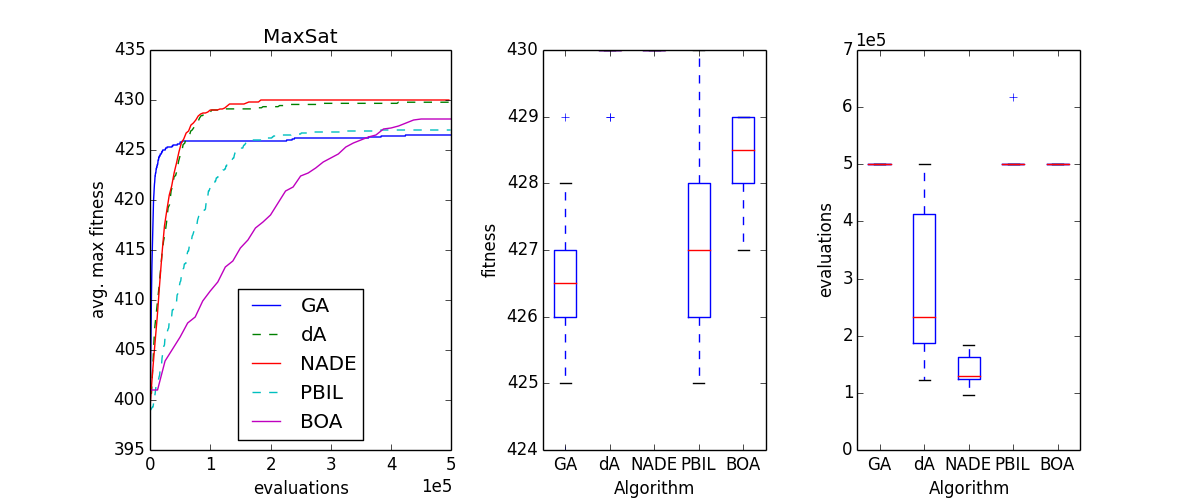
\includegraphics[scale=0.34]{results/maxsat.png}
    }
}
\subfigure[Knapsack (500 items, 1 constraint)]{
\makebox[0.5\textwidth]{
        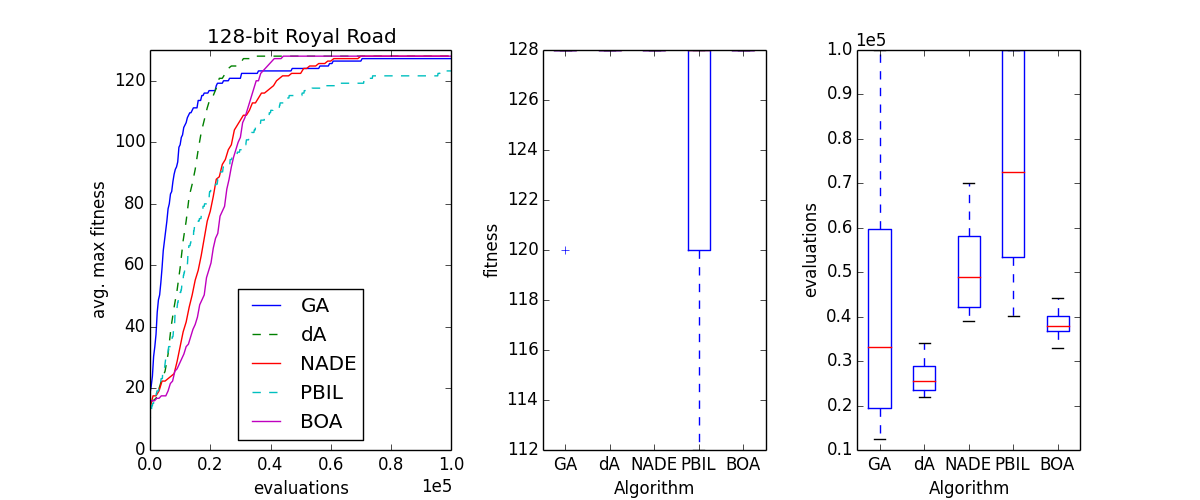
\includegraphics[scale=0.34]{results/royal_road.png}
    }
}
\subfigure[Weing Knapsack (105 items, 2 constraints)]{
\makebox[0.5\textwidth]{
        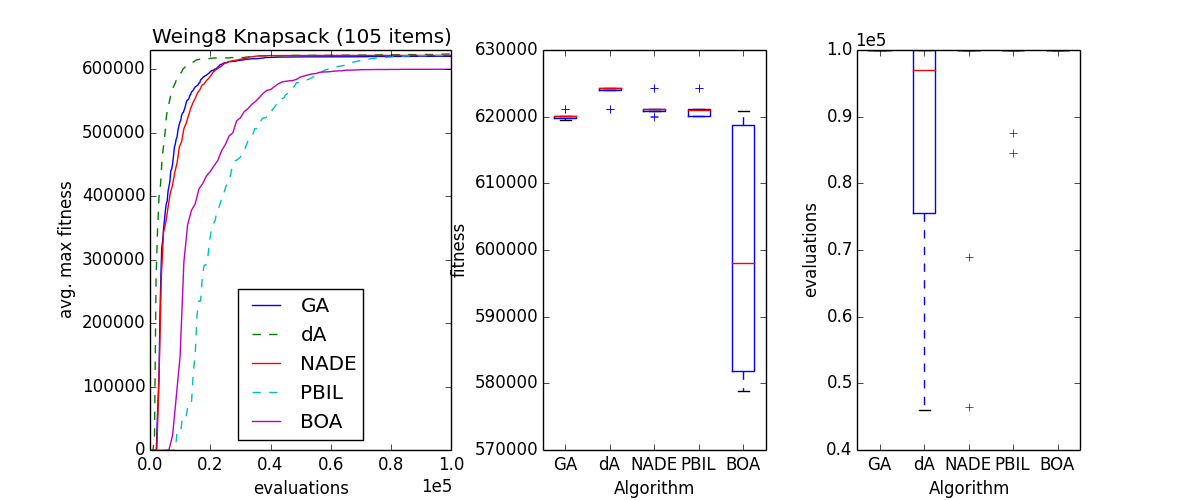
\includegraphics[scale=0.34]{results/knapsack_105.png}
    }
}
\caption[Optional caption for list of figures]{Showing results obtained by the different algorithms on MaxSat and Knapsack problems.}
\label{figure:results_plots1}
\end{figure}

\begin{figure}[t!]
\centering
\subfigure[128-bit Royal Road]{
\makebox[0.5\textwidth]{
        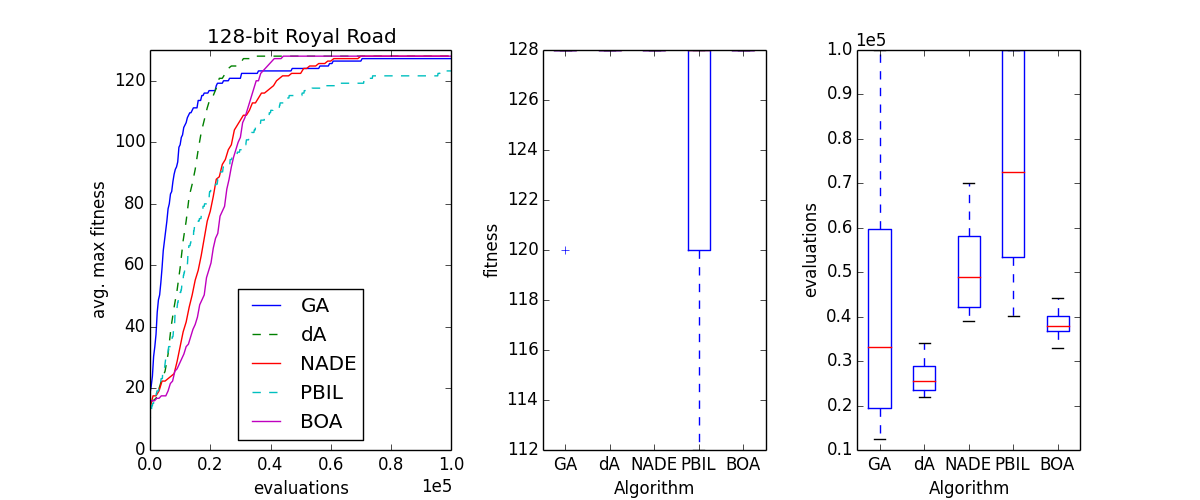
\includegraphics[scale=0.34]{results/royal_road.png}
    }
}
\subfigure[128-bit HIFF]{
\makebox[0.5\textwidth]{
        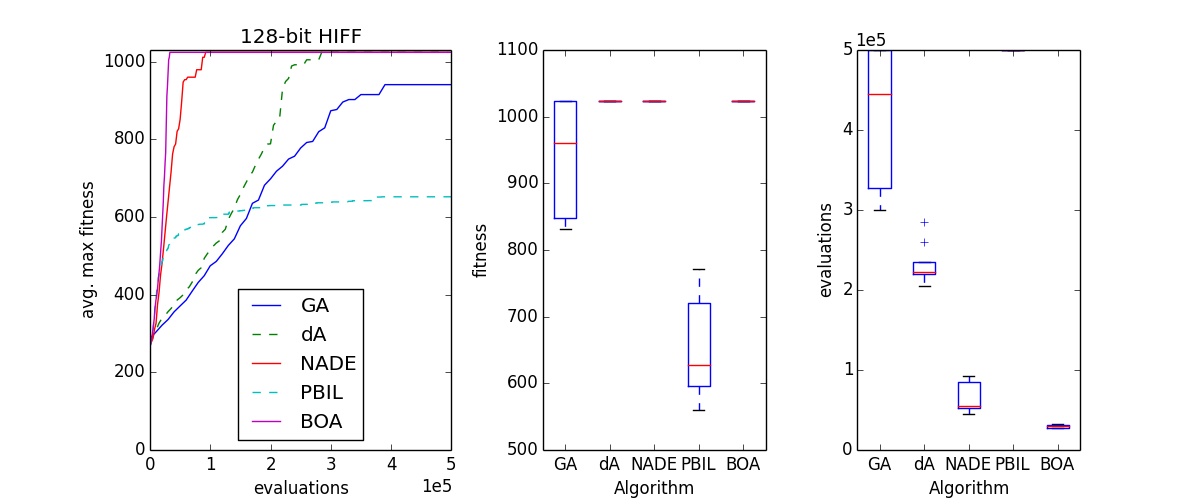
\includegraphics[scale=0.34]{results/hiff128.png}
    }
}
\subfigure[256-bit HIFF]{
\makebox[0.5\textwidth]{
        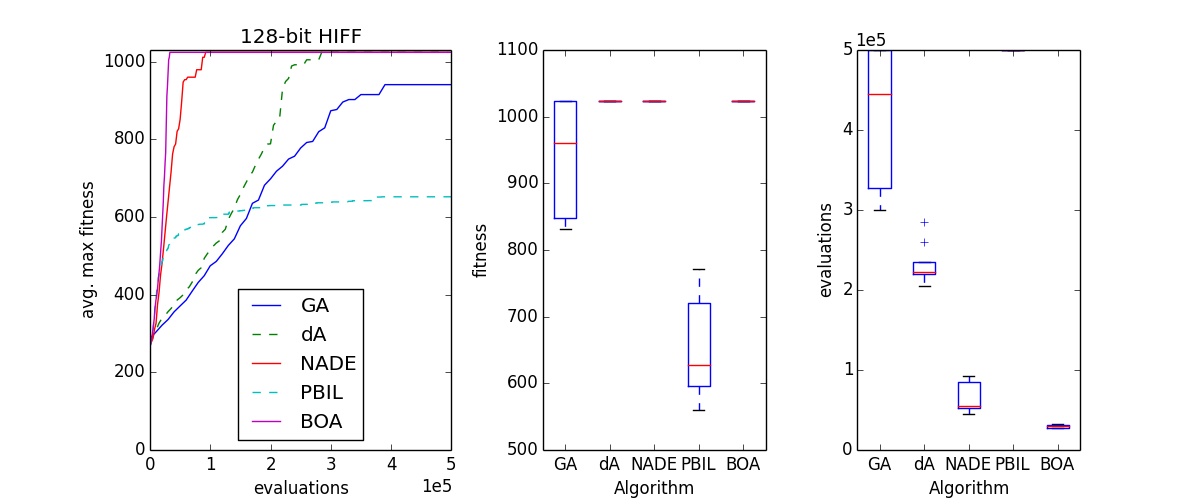
\includegraphics[scale=0.34]{results/hiff128.png}
    }
}
\caption[Optional caption for list of figures]{Showing results obtained by the different algorithms on Royal Road and HIFF problems.}
\label{figure:results_plots2}
\end{figure}
GA-dA is the clear winner on both knapsack problems. On the 500-item instance it is the only algorithm that locates the optimal solution and on the Weing8 instance (which has two constraints) it has a much greater success rate than the next best performer. On both problems it also improves its best solution much more quickly than the other algorithms. Both GA-NADE and BOA have much slower rates of improvement than GA-dA, although GA-NADE is considerably faster than BOA. BOA finds slightly better solutions than GA-NADE on the 500-item knapsack but performs considerably worse on the Weing8 instance.

On both tested HIFF instances BOA is the far better performer, solving the 128-bit problem twice as fast and the 256-bit instance three times faster than GA-NADE. In turn, GA-NADE is able to solve the 128-bit instance in half the evaluations required from GA-dA and a quarter as many on the 256-bit instance. GA-dA is better than the standard GA on this problem, solving it faster and more consistently. The GA is not able to solve the HIFF instances on every trial, although it can locate the optimal solution while PBIL cannot.

GA-dA displays the best performance on the Royal Road problem, consistently solving it within a small number of evaluations. The next best is the GA which can solve it more quickly but produces a much greater variance in discovery time. BOA is able to solve the problem much faster on average than GA-NADE, with low variance in terms of the number of evaluations taken to solve the problem.

\section{Discussion}

\subsection{Algorithmic Comparison}
The results presented in the preceding section demonstrate that the denoising autoencoder (GA-dA) and NADE (GA-NADE) methods perform well across a number of difficult discrete problems. GA-dA outperforms the other methods on both knapsack problems and the Royal Road and GA-NADE is the only algorithm that is able to consistently solve the MaxSat problem instance. GA-dA outperforms a GA on all test problems in terms of the quality of the final solution and/or the number of evaluations required. GA-NADE outperforms a GA on all of the problems apart from the Royal Road and the 500-item knapsack where they are not significantly different. BOA outperforms both neural network methods on the HIFF problems. It also outperforms GA-NADE on the Royal Road and Knapsack-500 problems but not on the others. This suggests that the BOA EDA method is better able to discover the type of dependancy present in the HIFF problem. GA-NADE performs considerably better than GA-dA, which suggests that the Bayesian Graph-based generative model is well-suited to discovering the structure in the search space present in this problem. The poor performance of PBIL on the HIFF problem indicates that a model capable of learning complex multivariate dependencies is needed. The structure learnt by GA-dA allows it to significantly outperform the GA but it is much slower than BOA or GA-NADE. 

A MaxSat problem is difficult because there are a large number of interdependencies between variables and solving subproblems in the form of individual clauses can lead you away from the optimal solution (ref\ref{}). GA-NADE is able to solve this problem consistently while BOA is not. This problem could be well suited to the NADE model which assumes a dependency between every variable - each variable is either a parent or a child of another. Thus a complex joint distribution of the variables is learnt. The dA is also able to learn multi-variate dependency with the potential advantage of having no precedence constraints. The tested implementation of BOA restricts each node to have at most 2 parents, which may adversely affect its ability to find solutions to this problem. Increasing this limit is prohibitively expensive.

The knapsack problems are interesting for two reasons, they have have real-world uses in resource management and they do not have obvious linkages. A 3-CNF MaxSat problem is complex because individual variables are present in multiple clauses and changing one variable can have a large impact on the fitness of the sequence. Due to the nature of the constraint handling of these knapsack problems, here a small change can have a huge impact on fitness. If a solution changes from being under to over capacity, its value will swing from positive to negative. If there were no constraints, a knapsack problem would reduce to a MaxOnes problem and all variables would be fully independent. Variables can still be treated independently, which effectively will give a higher probability to high value or high density items. Given more constraints the dependencies between groups of variables become more complex as certain combinations of items are required in order to satisfy the constraints. In terms of the rate of improvement, PBIL performs much better on the single constraint knapsack problem but takes much longer to get close to the optimal solution compared to GA-NADE, GA-dA and the GA. BOA has a much slower improvement rate on the Weing8 instance and does not find as good solutions. The GA uses a high crossover rate of 0.5 and thus swaps a large number of partial solutions. GA-dA has the fastest improvement rate and the highest mean score on both knapsack problems. This may be the type of problem for which it is best suited, as the dA has no ordering constraints, can capture dependencies between large groups of variables and, importantly, mutate around these solutions.

GA-dA is also the fastest consistent solver of the 128-bit Royal Road Problem. This problem is famous because it was used to identify the hitch-hiking phenomenon that can adversely affect the performance of GAs. For an EDA to perform well on this problem, it has to build a model that learns that either the blocks are independent or that every variable is independent. PBIL suffers on this problem by falling into a local optima where certain variables have a very low probability of outputting a one. At this point it becomes very unlikely that certain subproblems will be solved. At the point of solving, BOA has learnt a model where every variable is independent. We will look more closely at the models produced by GA-dA and GA-NADE in the next section but GA-NADE clearly learns a complex relationship between variables that does not exist in the real problem. GA-dA hones in a very small part of the sub-space, which allows it to quickly find the optimal solution.
%
%- Royal Road has lots of noise that may be fitted by NADE
%- Knapsacks have dependency but are also independent
%- In next section make a big deal about ordering
%- In previous section about BOA make a big deal about 2 parents
%- Stats
%- 
%Across all test problems PBIL was consistently the worst performer. 
\begin{figure}[t!]
\centering
\subfigure[A reduced view of each sub-partition for each sample]{
\makebox[1.0\textwidth]{
        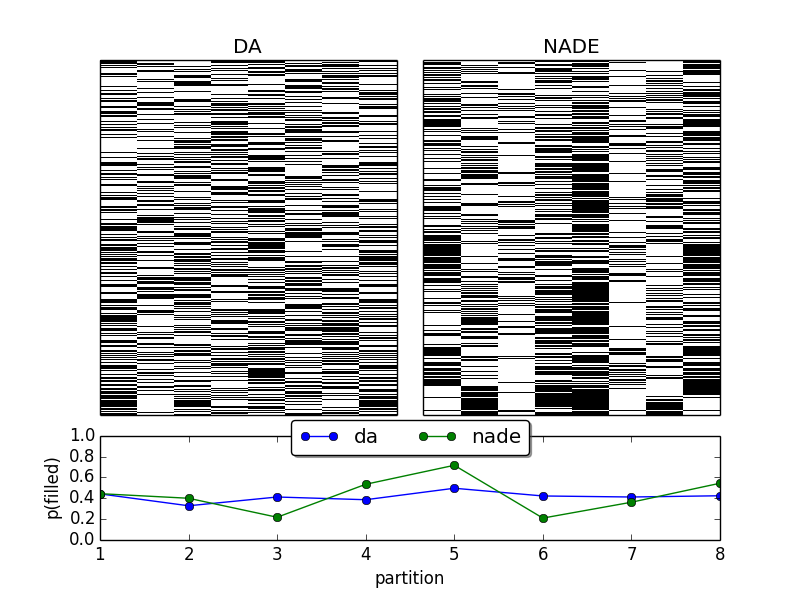
\includegraphics[scale=0.5]{nade-vs-da-wide.png}
    }
}
\subfigure[A reduced view of each sub-problem for each sample]{
\makebox[1.0\textwidth]{
        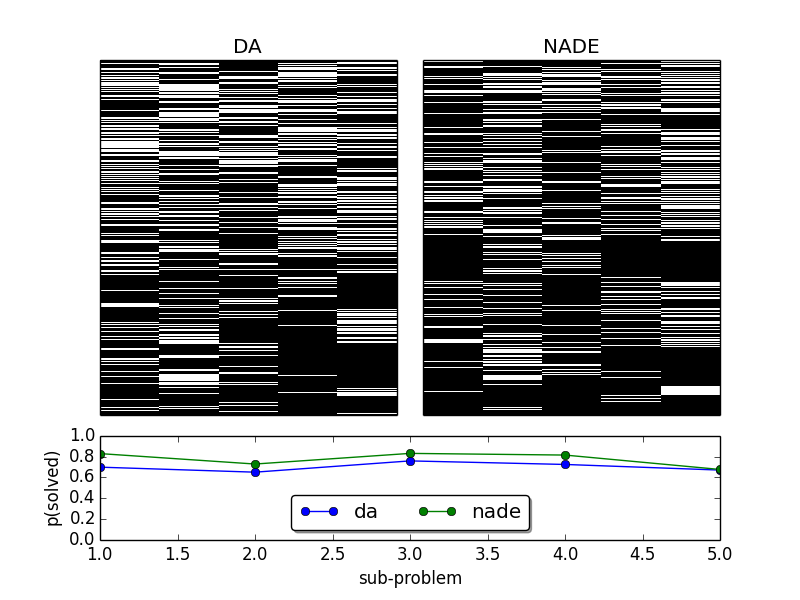
\includegraphics[scale=0.5]{nade-vs-da-narrow.png}
    }
}
\caption[Optional caption for list of figures]{Showing samples from the dA and NADE on the Royal Road with Linkages problem.}
  \label{fig:nade_vs_da1}
\end{figure}

\begin{figure}[t!]
\centering
    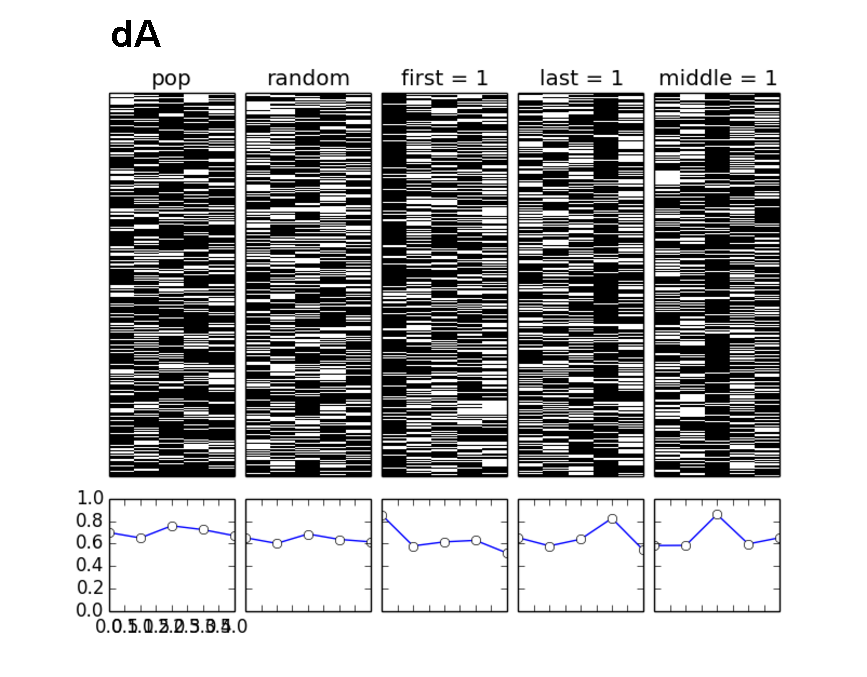
\includegraphics[scale=0.7]{da_croad.pdf}
  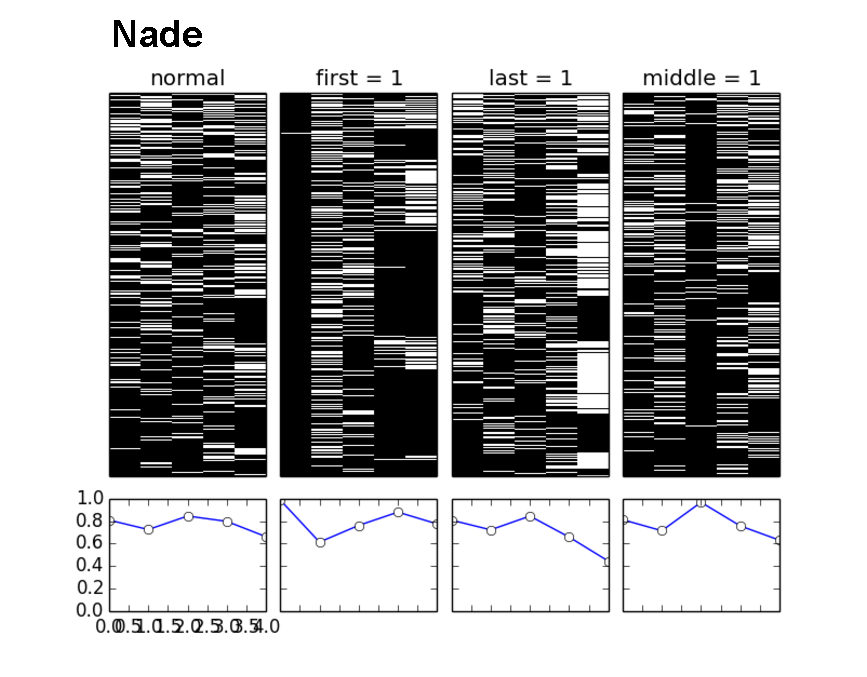
\includegraphics[scale=0.7]{nade_croad.pdf}
  \caption{}
  \label{fig:nade_vs_da2}
\end{figure}

\subsection{Neural Network Methods Comparison}

There are clear differences in the performance of the two Neural Network based algorithms, with GA-NADE performing much better than GA-dA on the HIFF and MaxSat problems but significantly worse on the others. The two methods discover structure in solution space in considerably different ways, with GA-NADE creating a generative model in the form of a Bayesian graph and GA-dA through a compressed encoding of promising solutions. In this section we will first investigate the differences between the NADE and Autoencoder models on a specially designed function and then provide further analysis on a selection of the problems from the results section above.

\subsubsection{A Royal Road with Linkages}
A new objective function has been devised based on Mitchell et al.'s Royal Road [\cite{mitchell}]. A solution consists of \(n\) non-overlapping partitions, \(p_i i\in{[1\ ... \ n]}\), of size \(2k\). \(p_i\) is further divided into two non-overlapping partitions of size \(k\), \(\hat{p}_{iL}\) on the left side and \(\hat{p}_{iR}\) on the right. If each bit in \(\hat{p}_{iL}\) is equal to 1 and each bit in \(\hat{p}_{iR}\) is equal to 0, 1 is added to fitness. Alternatively, a 1 is added to fitness if each bit in \(\hat{p}_{iL}\) is equal to 0 and each bit in \(\hat{p}_{iR}\) is equal to 1. Finally, an additional 1 is added to fitness if every bit in \(\hat{p}_{1L}\) and \(\hat{p}_{nR}\) are equal to 1, or if every bit in \(\hat{p}_{1L}\) and \(\hat{p}_{nR}\) is equal to 0, where \(i=1\) signifies the first partition and \(i=n\) the last. An example is given for a 24-bit sequence in figure ?. This fitness function has been invented to explore how the algorithms deal with dependency between blocks of variables. There is linkage between the first and second halves of each partition, which is referred to below as `local-linkage', and between the first \(k\) and the last \(k\) bits in the string, referred to as the `global-linkage'.

GA-NADE and GA-dA are applied to a 32-bit version of this problem (\(k=4,n=4\)), both using a population size of 500. Samples produced by the models at the point that the optimal solution is found are explored in figures ~\ref{fig:nade_vs_da1} and ~\ref{fig:nade_vs_da2}. In figure ~\ref{fig:nade_vs_da1}(a), samples have been reduced from 32 dimensions to 8, by displaying only the sub-partitions. If more than 2 bits in a sub-partition are equal to 1, the corresponding element in the string in the figure is assigned a 1, with a 0 otherwise. Underneath each figure a plot shows the overall bias, the probability of a sub-partition consisting of all 1s or all 0s, averaged across the samples. Figure ~\ref{fig:nade_vs_da1}(b) shows, for each sample, which of the four partitions have been solved (sub-problems 1 - 4), and whether every bit in \(\hat{p}_{1L}\) and \(\hat{p}_{nR}\) is equal to 1, or if every bit in \(\hat{p}_{1L}\) and \(\hat{p}_{nR}\) is equal to 0 (sub-problem 5). Therefore it shows which local-linkage sub-problems have been solved and whether the global-linkage problem has also been solved.

Figure ~\ref{fig:nade_vs_da1} shows 500 samples from the dA and NADE, with the dA using the final population as input. In terms of sub-partition behaviour, the NADE exhibits a much clearer bias, with sub-partition 3 biased towards 0s and 4 biased towards 1s, and sub-partition 5 biased towards 1s and 6 biased towards 0s. This shows that the NADE has produced a peaked distribution in certain parts of solution space. Looking at the solution of sub-problems in figure ~\ref{fig:nade_vs_da1}(b), the samples generated by both algorithms solve the problems in all of the partitions with high probability. NADE displays a slightly higher probability of solving the local-linkage problems in partitions but both have an equal probability of solving sub-problem 5.

We have seen in Figure \ref{fig:nade_vs_da1} that although the algorithms produce samples from different distributions they have similar probabilities of solving the sub-problems. In figure~\ref{fig:nade_vs_da2} we now probe the models to investigate the structure that has been learnt. Figure \ref{fig:nade_vs_da2}(a) shows sub-problems solved by 50,000 samples from the dA given different input conditions. The first condition is the same as in figure \ref{fig:nade_vs_da2}, using the final population as input to the model. The second condition uses input strings sampled from a uniform random distribution. The third, fourth and fifth conditions also use samples from a uniform random distribution for input but fix the sub-partitions \(\hat{p}_{1L}\) (referred to as \(c_{first}\)),  \(\hat{p}_{3L}\) (\(c_{middle}\)), and \(\hat{p}_{4R}\) (\(c_{last}\)) to equal all ones, respectively.

Using input from a uniform random distribution we see that sub-problem solutions follow a similar distribution to using the final population as input, but the probability of solving a sub-problem is slightly lower. With condition \(c_{first}\) there is an increase in the frequency of solutions to the first sub-problem, showing that the algorithm increases the probability of setting the sub-partition on the right to all zeroes, and suggesting that it has learnt the local-linkage in this partition. However, the probability of solving the global-linkage between the first and last sub-partitions, \(\hat{p}_{1L}\) and \(\hat{p}_{4R}\), has decreased, although not drastically. Similar behaviour is seen with \(c_{last}\), where the probability of solving the sub-problem in the last partition is increased, however this leads to a small decrease in the probability of solving the global-linkage. For \(c_{middle}\) we see an increase in solving the third subproblem (which is independent from the other partitions) without any noticeable change in the probability of solving the other sub-problems.

In figure \ref{fig:nade_vs_da2}(b), we perform a similar probe on the NADE. Here, the first plot shows samples from the model with no bias applied to probabilities. The second, third and fourth plots sample from the same NADE model but fix the probability of a 1 in the sub-partitions \(\hat{p}_{1L}\) (\(c_{first}\)), \(\hat{p}_{3L}\) (\(c_{middle}\)), and \(\hat{p}_{4R}\) (\(c_{last}\)) to be equal to 1, respectively. In constrast to the dA, with the NADE the \(c_{first}\) condition increases the probability of solving the first subproblem to almost 1, while also greatly increasing the probability of solving the long range dependency of the last sub-problem. The condition \(c_{middle}\) greatly increases the probability of solving the middle sub-problem while not affecting the distribution of solutions to the other sub-problems. Finally, the condition \(c_{last}\) has a negative effect, decreasing the probability of solving the last two subproblems, and affecting the long-range dependency particularly badly.

The samples displayed in figure \ref{fig:nade_vs_da2} provide an interesting insight into the differences between the two models. The condition \(c_{first}\) provides a much greater performance increase with the NADE than with the dA. Setting the left half of the first partition to all ones means that the right half of the first partition must contain all zeros, the right half of the last partition must also contain all zeros and the left half of the last partition must contain all ones. This means that a complex sequence of linkages must be learnt. Figure \ref{fig:nade_vs_da2} clearly demonstrates that the NADE is able to completely capture both the local and global linkages, while the dA only captures the local. However, the dA has certainly learnt complex dependencies, as in the \(c_{last}\) condition, while there is a small decrease in solving the long range dependency, it is not anywhere near as drastic as that displayed by the NADE, which means that it is influencing the first sub-partition. The dA does not suffer from ordering constraints, while the NADE does, therefore fixing the last sub-partition cannot influence the probabilities of the variables in earlier partitions. This implies that ordering could have a large influence on the performance of the NADE, which is a topic for further investigation. There is more flexibility in biasing the variables in the dA, which could be utilised to further guide the search process.
\begin{figure}[t!]
\centering
\subfigure[Showing the distribution of the mean distances from their 5 nearest neighbours and the fitnesses of 50,000 samples from the dA and NADE at the point that the optimal solution is found]{
\makebox[1.0\textwidth]{
        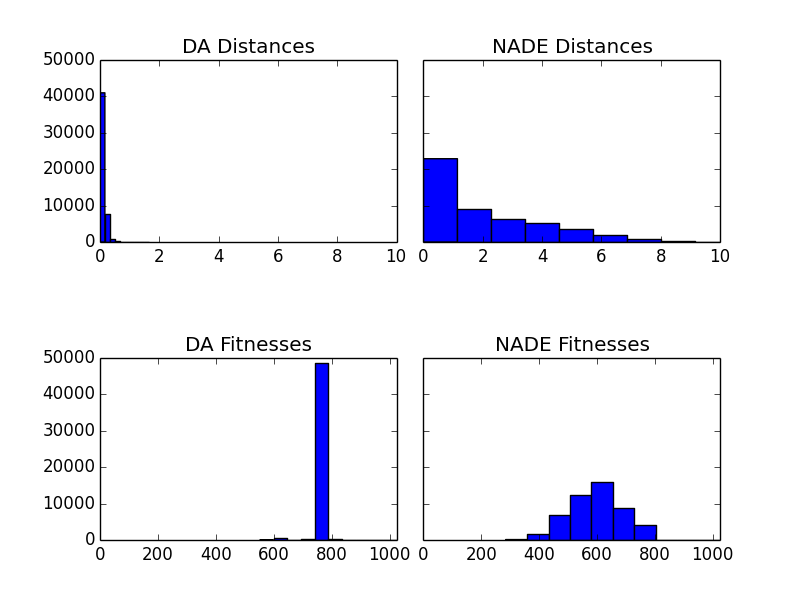
\includegraphics[scale=0.4]{hiff_hist.png}
    }
}
\subfigure[Showing 2,000 random samples (first row) and the probability of a 1 at each locus averaged over 50,000 samples (second row).]{
\makebox[1.0\textwidth]{
        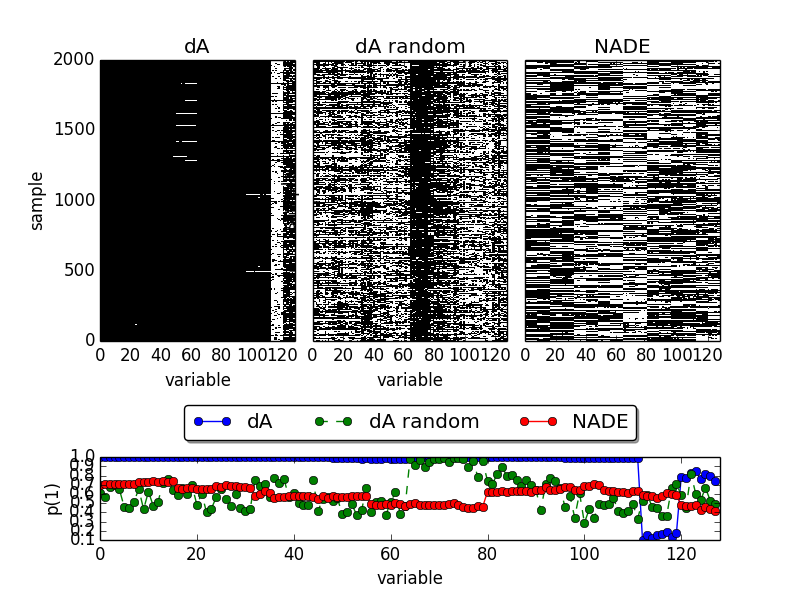
\includegraphics[scale=0.4]{results/hiff_sample_probs_random.png}
    }
}
  \caption{Showing statistics from samples from the dA and NADE models on the 128-bit HIFF.}
  \label{fig:results_hists1}
\end{figure}

\begin{figure}[t!]
\centering
\subfigure[Showing the distribution of the mean distances from their 5 nearest neighbours and the fitnesses of 50,000 samples from the dA and NADE at the point that the optimal solution is found]{
\makebox[1.0\textwidth]{
        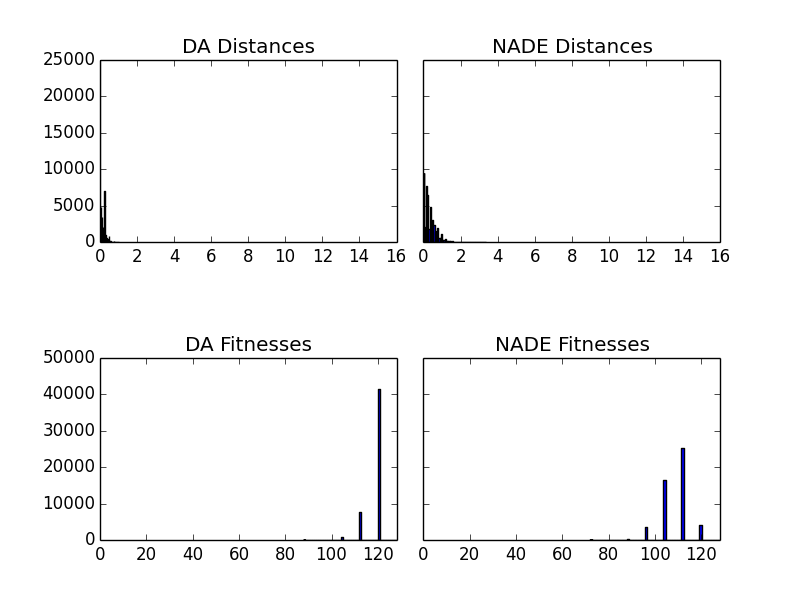
\includegraphics[scale=0.4]{results/royal_road_hist.png}
    }
}
\subfigure[Showing 2,000 random samples (first row) and the probability of a 1 at each locus averaged over 50,000 samples (second row).]{
\makebox[1.0\textwidth]{
        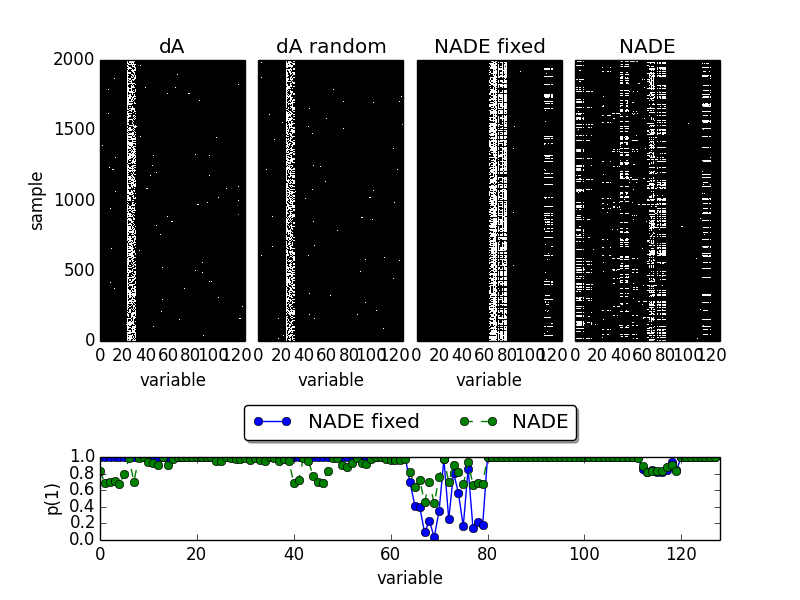
\includegraphics[scale=0.4]{results/rr_sample_probs_random.png}
    }
}
  \caption{Showing statistics from samples from the dA and NADE models on the Royal Road.}
  \label{fig:results_hists2}
\end{figure}

\begin{figure}[t!]
\centering
\subfigure[Showing the distribution of the mean distances from their 5 nearest neighbours and the fitnesses of 50,000 samples from the dA and NADE at the point that the optimal solution is found]{
\makebox[1.0\textwidth]{
        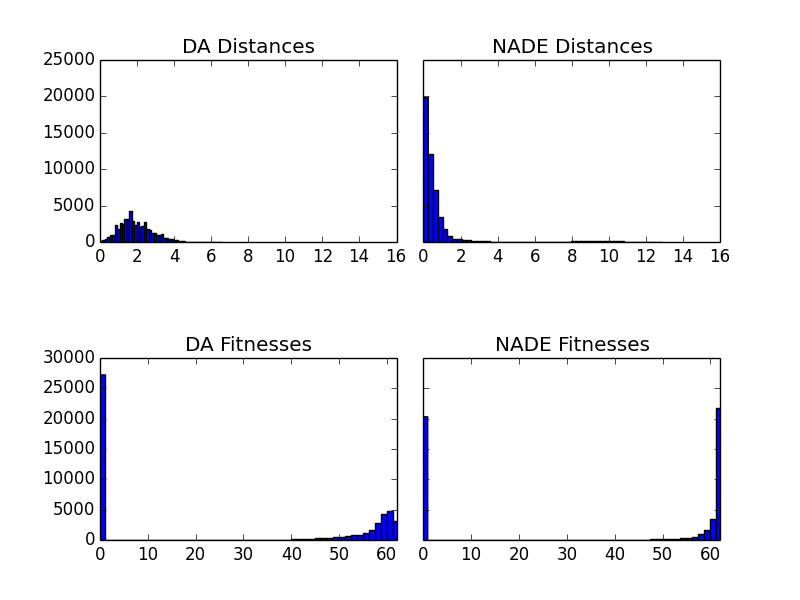
\includegraphics[scale=0.4]{results/knapsack_hist.png}
    }
}
\subfigure[Showing 2,000 random samples (first row) and the probability of a 1 at each locus averaged over 50,000 samples (second row).]{
\makebox[1.0\textwidth]{
        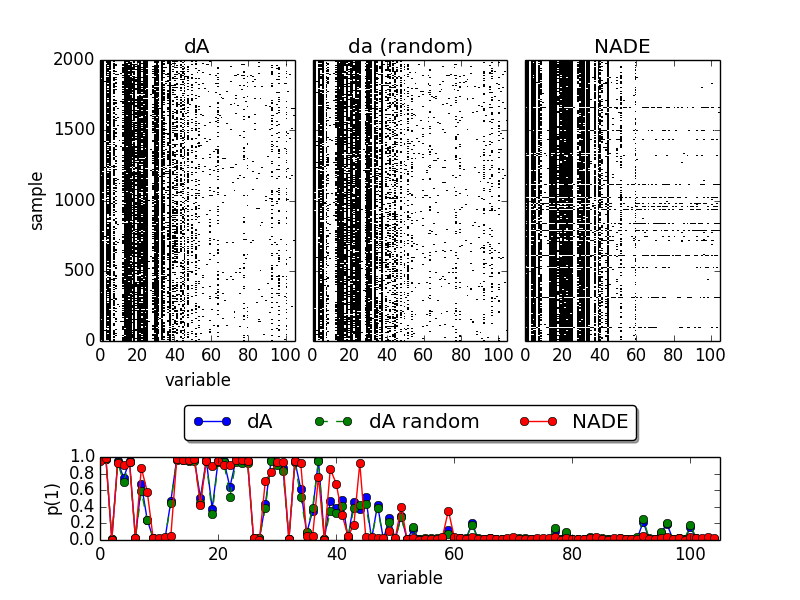
\includegraphics[scale=0.4]{results/knapsack_sample_probs_random.png}
    }
}
  \caption{Showing statistics from samples from the dA and NADE models on the Royal Road.}
  \label{fig:results_hists3}
\end{figure}

\subsubsection{Tested Problems}

We will now take a closer look at a selection of the test problems where there was a marked difference between GA-dA and GA-NADE: HIFF-128, the Royal-Road and Weing8. Figure \ref{fig:results_hists1}(a) shows the distribution of the mean distances from their 5 nearest neighbours and the fitnesses of 50,000 samples from the dA and NADE at the point that the optimal solution is found on HIFF-128. Here we see that there is much greater diversity in the samples produced by the NADE, while the dA has a much more peaked distribution. This can be partly explained by the fact that the dA does not use niching on this problem (which improved its performance). On this problem, most of the dA's solutions are small mutations around the local optima of 784, while the NADE produces a much more diverse set of samples. Looking at a selection of samples in \ref{fig:results_hists1}(b), we see that the dA model using the population as input is extremely peaked, with almost all variables in the string set to 1 apart from the last 16 bits. Using input sampled from a uniform random distribution produces a more varied distribution of solutions, although the fitness of the samples is not as high. The NADE produces a much less biased distribution of samples, which explains its better performance on this problem. Of particular interest is that samples from the NADE contain partial solutions from both the `all ones' and `all zeroes' global optima, while the dA concentrates on the `all ones' optima. This implies that NADE is better suited towards capturing the distribution of multi-modal search spaces.

The distribution of samples from the dA is similar for the Royal Road problem, with 15 of the 16 8 bit partitions almost always being all ones and mutations around a single unfilled partition. Although the NADE appears to produce more diverse samples, the distribution is peaked with a very low probability of a one on bits 64 - 80 (partitions 8 and 9). Fixing \(p(x_i)=1\) for the first 64 bits (\(i\in{[1\ ...\ 64]}\)) in the NADE modelling when sampling increases \(p(x_i)=0\) for \(i\in{[64\ ...\ 80]}\). This shows that a false dependency has been learnt linking earlier parts of the bit string to partitions 15 and 16, and it makes it very unlikely that the optimal solution will occur in a sample. This could be due to the topology of the dependency graph that the NADE is tied to. For the dA model, we see in this case that there is very little difference between using input from a random distribution or from the population, which is due to the high level of corruption (\(p(c)=0.9\)).

For the Weing8 knapsack problem instance, the histograms in figure \ref{fig:results_hists3}(a) show that the NADE produces slightly less diversity in its samples. The fitnesses of the samples are also heavily skewed towards very high scoring. Both models produce a large number of infeasible (and thus low scoring) samples. The raster plots in figure \ref{fig:results_hists3}(a) indicate that both models concentrate on similar solutions, with a peaked response to many variables on the left side of the string (items < 50). As indicated in the aggregate plot in \ref{fig:results_hists3}(b), the NADE has a more peaked response to many variables than the dA. We see in the raster plot that there are a number of samples from the NADE that use fewer items from the left side of the string and more from the right side (leading to the appearance of lines in the plot). This suggests that, similarly to the HIFF example, the NADE can model a multi-modal distribution, which could be useful for multi-modal search spaces or multi-objective optimisation. The corruption level is relatively high in the dA in this example (\(p(c)=0.25\)), and there is only small differences between using the population and a random sample as input to the model. However, using the population does increase the probability of certain variables in a number of positions.
 
\subsection{Areas for Further Investigation}
In this paper we have demonstrated how the dA and NADE models can be incorporated into an evolutionary search. Both models outperform a GA on number of problems (the dA is never beaten by a GA) as well as PBIL and BOA on certain problems. There are a number of areas that are currently being investigated that could potentially improve performance. Both models are trained online, and we have seen in the previous section that a bias creeps into the models. For example, in the Royal Road problem the NADE has a strong bias towards the bits in two partitions being set to 0, keeping it in a local optima for a long time. Training online allows search space structure discovered earlier in the search process to be reused later. It also helps to keep down the computational cost of model building. However, rebuilding the models either at certain predefined intervals, at every iteration or when probabilities begin to peak could reduce sample bias and improve the performance of the algorithm. As an aside, there could be another benefit to training online, which is the potential for transfer of the models between different related instances of the same class of problem. The question of transfer learning - can building a model to solve one task help improve performance on another? - has not been answered by the EDA community, although recent work has made a start (e.g. \cite{hauschild2012using}). Preliminary investigations suggest that using a dA, information learned in one task can be retained and recombined with that learnt in a second task to produce an across the board speed up on the third task in the sequence. Careful experimentation is needed to discover which types of problem can use machine learning techniques to transfer knowledge between unique instances and speed up optimisation as more examples are encountered.

In the last decade there has been a resurgence of interest in neural network-based methods, spurred by so called `deep architectures'. Both the dA and NADE could potentially benefit from the hierarchical features supported by deep networks and this needs to be investigated further. A potential problem with the NADE model is the precedence ordering of variables, which could have a great effect on the quality of the learnt distribution, as well as the training time. There are several paths that could be taken in this direction, for example having multiple models being learnt in parallel or using alternate methods to learn Bayesian graphs at certain points in the search process and using the discovered ordering for the NADE model.

\subsection{Real Valued, Mixed Integer and Multi-objective Problems}
Both the NADE and dA can be modified to work with continuous or mixed-integer domains, providing an advantage over other discrete only EDA methods.

\section{Conclusion}
We have presented a novel stochastic evolutionary algorithm based on two neural network models that provide a distribution of mutated samples. Training online, using the best found genotypes, the models are able adaptively learn an exploration distribution, which guides it towards optimal solutions on difficult problems such as the 256-bit HIFF, regularly outperforming a Genetic Algorithm and other EDA methods on a number of problems.
\small

\bibliographystyle{apalike}
\bibliography{ecjsample}


\end{document}
